\documentclass[11pt, english, fleqn, DIV=15, headinclude]{scrartcl}

\usepackage[bibatend, color]{header}

\usepackage{pdflscape}
\usepackage[section]{placeins}

\hypersetup{
    pdftitle=
}

\subject{physics760 Computational Physics}
\title{Analysis of $\piup$-$\piup$ lattice QCD scattering data}
%\subtitle{}
\author{
    Martin Ueding \\ \small{\href{mailto:mu@martin-ueding.de}{mu@martin-ueding.de}}
}

\begin{document}

\maketitle

\begin{abstract}
    % TODO
\end{abstract}

\tableofcontents

\newpage

\section{Data generation}

\subsection{Metropolis algorithm}

\subsection{Correlation functions}

\section{Analysis methods}

Figure~\ref{fig:analysis-flow} shows the data flow in the analysis. This
section will go through the whole analysis in the order of the flow chart. The
methods used will be explained along the way when they are needed.

\begin{figure}[htbp]
    \centering
    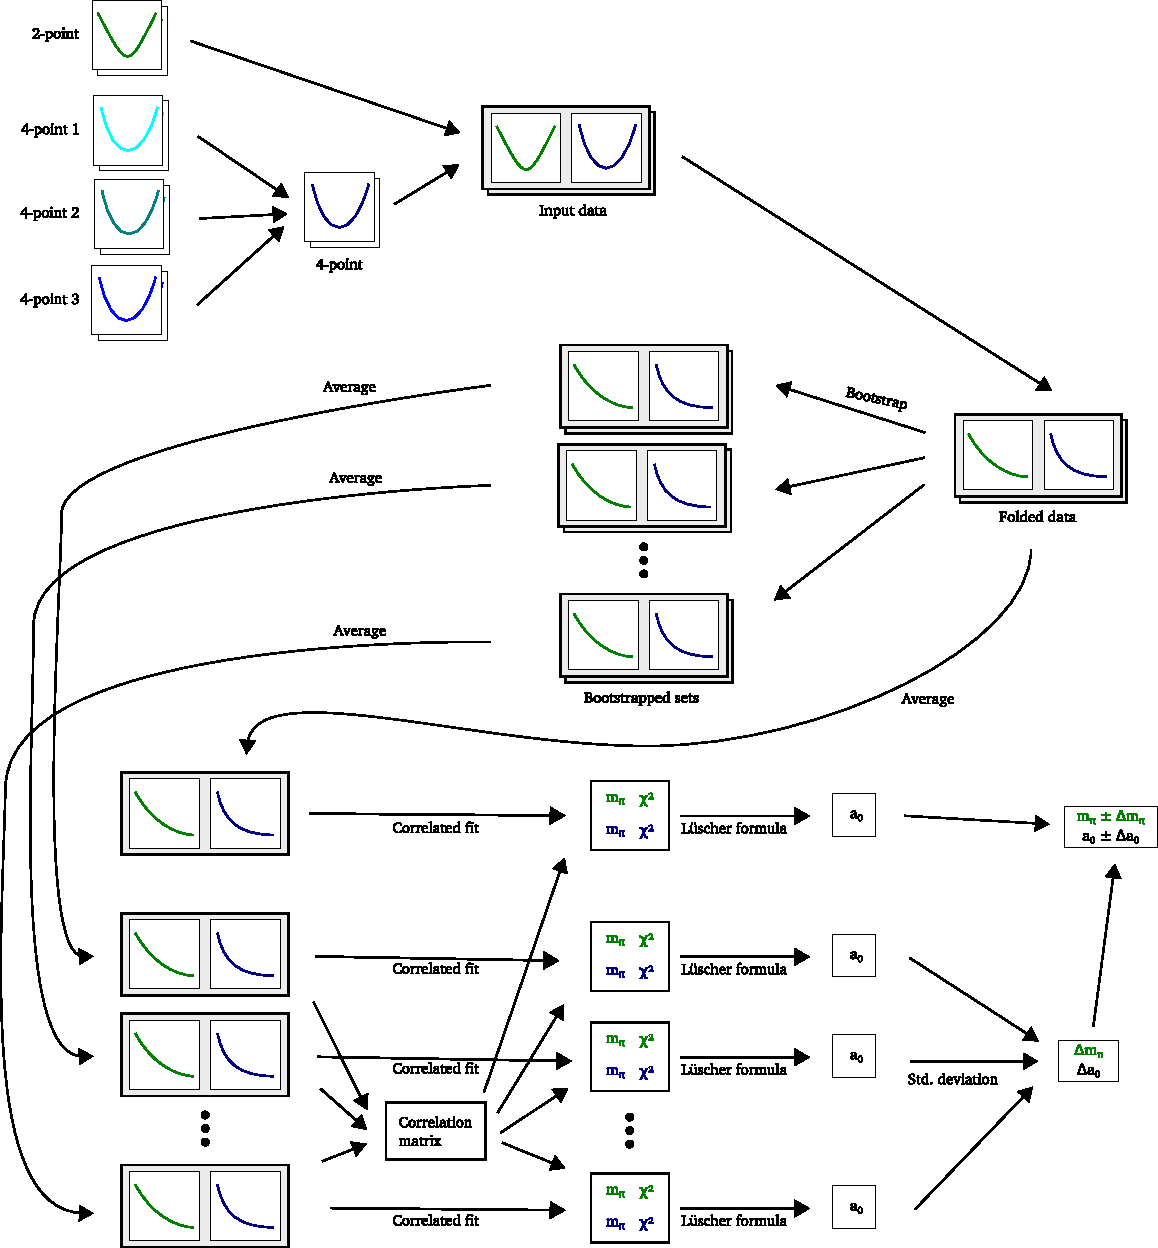
\includegraphics[width=\linewidth]{sketches/Zeichnung.pdf}
    \caption{%
        Data flow in the analysis.
    }
    \label{fig:analysis-flow}
\end{figure}


\subsection{Import data}

The data that I was given is organized in different ensembles (like A30.32,
A100.24). For each ensembles, multiple configurations were simulated. The
output of each configuration is a two-point correlation function $C_\piup(t)$
and three four-point correlation functions $C_{\piup\piup}^{(i)}(t)$. Those
three different contractions are combined into a single
$\piup\piup$-correlation function:
\[
    C_{\piup\piup}(t) = C_{\piup\piup}^{(1)}(t) + C_{\piup\piup}^{(2)}(t)
    - 2 C_{\piup\piup}^{(3)}(t).
\]

Some of the ensembles had multiple versions of the data in it. I analyzed all
of them sorted by file name. In the tables, you will find the ensembles
multiple times, those are the different versions.

The number of configurations in each ensemble is called $N$.

\subsection{Bootstrap}

All error estimation is done with the bootstrap method. The number of bootstrap
samples $R$ was set to $R = 3N$.

\subsection{Correlated fit}

The computed masses are shown in table~\ref{tab:masses}.

\subsection{Scattering length}

The computed scattering lengths are shown in table~\ref{tab:masses}.

\section{Results}

\begin{table}
    \centering
    \begin{tabular}{lSSS}
        ensemble & {$m_{\piup}$}  & {$m_{\piup\piup}$} & {$a_0$} \\
        \midrule
        A100.24  & 0.22238 +- 0.00023  & 0.45125 +- 0.00052 & -1.346 +- 0.029 \\
        A100.24  & 0.22233 +- 0.00040  & 0.45083 +- 0.00095 & -1.287 +- 0.132 \\
        A100.24  & 0.22239 +- 0.00024  & 0.45111 +- 0.00053 & -1.316 +- 0.039 \\
        A30.32   & 0.12416 +- 0.00055  & 0.25135 +- 0.00144 & -0.904 +- 0.273 \\
        A40.20   & 0.14779 +- 0.00078  & 0.31429 +- 0.00162 & -1.426 +- 0.052 \\
        A40.24   & 0.14447 +- 0.00052  & 0.29815 +- 0.00109 & -1.255 +- 0.051 \\
        A40.24   & 0.14453 +- 0.00031  & 0.29842 +- 0.00071 & -1.272 +- 0.051 \\
        A40.32   & 0.14126 +- 0.00022  & 0.28626 +- 0.00055 & -1.228 +- 0.092 \\
        A60.24   & 0.17275 +- 0.00052  & 0.35278 +- 0.00126 & -1.194 +- 0.112 \\
        A60.24   & 0.17279 +- 0.00048  & 0.35404 +- 0.00099 & -1.361 +- 0.091 \\
        A80.24   & 0.19930 +- 0.00024  & 0.40511 +- 0.00057 & -1.228 +- 0.043 \\
        B55.32   & 0.15553 +- 0.00022  & 0.31589 +- 0.00055 & -1.676 +- 0.117 \\
        D45.32   & 0.12047 +- 0.00046  & 0.25057 +- 0.00137 & -2.416 +- 0.205
    \end{tabular}
    \caption{%
        Computed masses from correlation functions.
    }
    \label{tab:masses}
\end{table}

\begin{table}
    \centering
    \begin{tabular}{lSSSS}
        ensemble & {$L$} & {$T$} & {$a_0 m_\piup$} & {$m_\piup/f_\piup$} \\
        \midrule
        A100.24 & 24 & 48 & -0.2993 +- 0.0066 & 2.77 \\
        A100.24 & 24 & 48 & -0.2862 +- 0.0292 & 2.77 \\
        A100.24 & 24 & 48 & -0.2927 +- 0.0088 & 2.77 \\
        A30.32  & 32 & 64 & -0.1122 +- 0.0339 & 1.86 \\
        A40.20  & 20 & 48 & -0.2107 +- 0.0077 & 2.11 \\
        A40.24  & 24 & 48 & -0.1813 +- 0.0074 & 2.03 \\
        A40.24  & 24 & 48 & -0.1839 +- 0.0074 & 2.03 \\
        A40.32  & 32 & 64 & -0.1735 +- 0.0131 & 2.06 \\
        A60.24  & 24 & 48 & -0.2063 +- 0.0194 & 2.32 \\
        A60.24  & 24 & 48 & -0.2351 +- 0.0157 & 2.32 \\
        A80.24  & 24 & 48 & -0.2448 +- 0.0087 & 2.55 \\
        B55.32  & 32 & 64 & -0.2607 +- 0.0182 & 2.34 \\
        D45.32  & 32 & 64 & -0.2911 +- 0.0248 & 2.49
    \end{tabular}
    \caption{%
        Lattice size of the ensembles together with computed quantities.
        These data points are also shown in figure~\ref{fig:result}. The pion
        decay constants are taken from
        \parencite[table~1]{Knippschild/Pi_Pi_Scattering}.
    }
    \label{tab:computed}
\end{table}

The results from table~\ref{tab:computed} are shown in figure~\ref{fig:result}.

\begin{figure}[htbp]
    \centering
    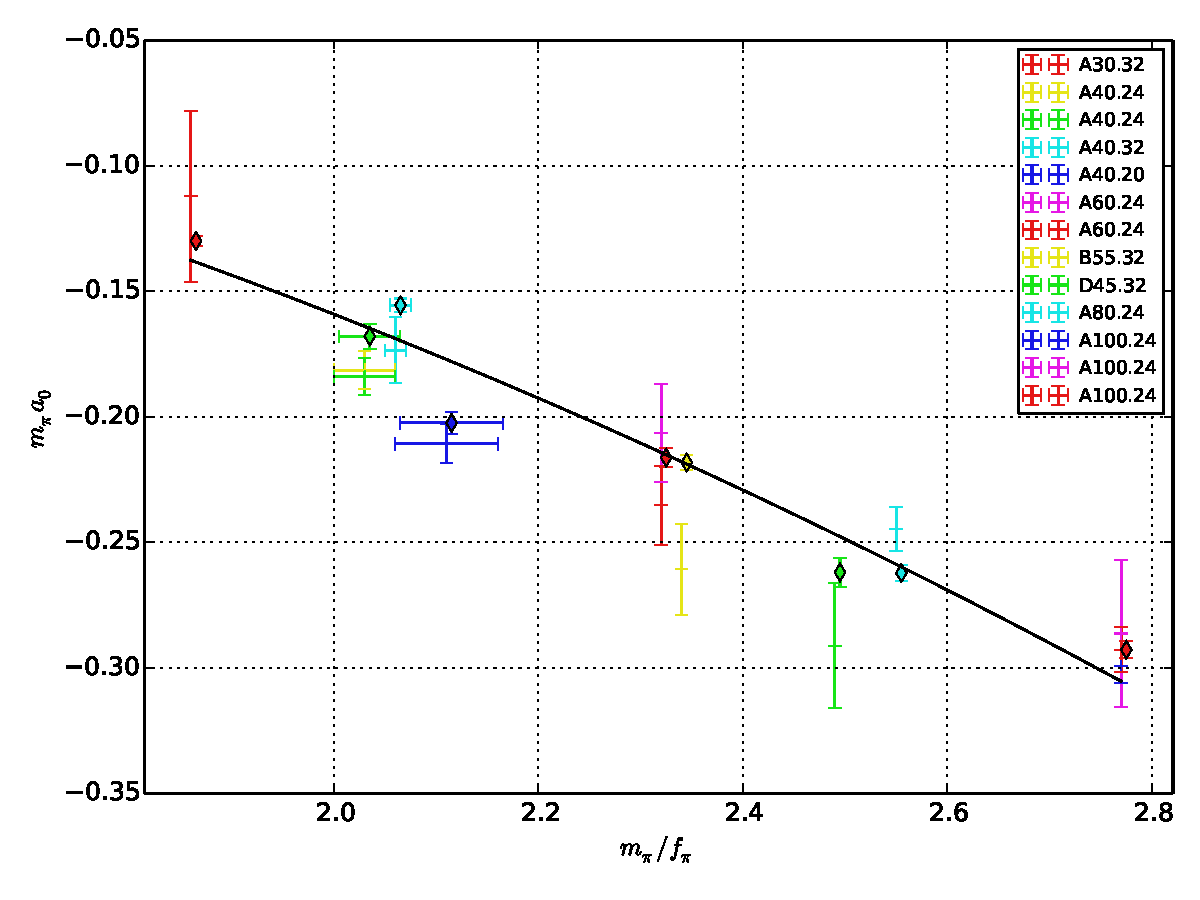
\includegraphics[width=\linewidth]{plots/result.pdf}
    \caption{%
        Results. Diamond data points are taken from draft paper.
    }
    \label{fig:result}
\end{figure}

\end{document}

% vim: spell spelllang=en tw=79
